\chapter{Sistemas complejos}
\section{Atractores}
\subsubsection{\large Simular y analizar el comportamiento complejo del atrayente de Lorenz} 
El descubrimiento de este atractor data de 1963, cuando Edward Norton Lorenz desarrolló un modelo matemático simplificado para la convección atmosférica. El modelo es un sistema de ecuaciones diferenciales ordinarias compuesto por tres ecuaciones ahora conocidas como las ecuaciones de Lorenz:
$$\left\{\begin{matrix}\frac{\mathrm{d}x}{\mathrm{d}t} &= \sigma (y - x), \\
	\frac{\mathrm{d}y}{\mathrm{d}t} &= x (\rho - z) - y, \\
	\frac{\mathrm{d}z}{\mathrm{d}t} &= x y - \beta z.\end{matrix}\right.$$
Normalmente se asume que los parametros $\sigma$, $\rho$, y $\beta$ son positivos. El interés en este modelo proviene de que para una seleccion de valores como $\sigma = 10$, $\beta = 8/3$ and $\rho = 28 $ el sistema exhibe un comportamiento caótico.

Si $\rho < 1$ entonces sólo hay un punto de equilibrio en el origen. Este punto además es un atractor global.

Si $\rho = 1$ entonces la en nuestra dinámica aparece una bifurcacion de pitchfork , y para  $\rho > 1 $ apareceen dos puntos de equilibrio, a saber $\left( \sqrt{\beta(\rho-1)}, \sqrt{\beta(\rho-1)}, \rho-1 \right) $ and $\left( -\sqrt{\beta(\rho-1)}, -\sqrt{\beta(\rho-1)}, \rho-1 \right). $ 
Este par de puntos será estable si : $\rho < \sigma\frac{\sigma+\beta+3}{\sigma-\beta-1}$

Como avanzábamos para valores como $\rho = 28$, $\sigma = 10$, and $\beta = 8/3$, el sistema de Lorenz tiene soluciones caóticas (es decir que, aunque no todas las soluciones son caóticas algunas de ellas si pueden presentar este comportamiento).

 Casi todos los puntos iniciales tenderán a un conjunto invariable que es lo que denominamos el atractor de Lorenz (véase figura:\ref{lorentz1}), cuya forma geométrica es reconocible. Este comportamiento caótico se refleja en la gran sensibilidad del atractor frente a cambios en las condiciones iniciales como se puede ver en la grafica \ref{lorentz2}.\textit{ Las graficas pertenecen a extractos de animaciones que pueden consultarse en github.}
 
 \begin{figure}
 	\centering
 	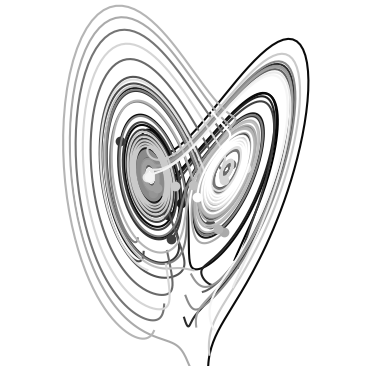
\includegraphics[width=8cm]{lorentz}
 	\caption{Atractor de Lorentz}
 	\label{lorentz1}
 \end{figure}
 \begin{figure}
 	\centering
 	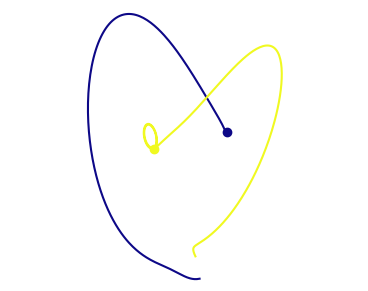
\includegraphics[width=8cm]{lorentz1}
 	\caption{Atractor de Lorentz: variacion respecto a condiciones iniciales}
 	\label{lorentz2}
 \end{figure}
 
 \subsubsection{\large Simular y analizar el comportamiento complejo del atrayente de Rossler} 
 
 El atractor de Rössler es el atractor del sistema de Rössler, un sistema de tres ecuaciones diferenciales ordinarias no lineales estudiadas por Otto E. Rössler. Estas ecuaciones diferenciales definen un sistema dinámico del tiempo-continuo que muestra dinámicas caóticas asociadas con las propiedades fractales del atractor:
 $$\left\{\begin{matrix}\frac{dx}{dt} &= -y - z \\
 \frac{dy}{dt} &= x + ay, \\
 \frac{dz}{dt} &= b + z(x-c).\end{matrix}\right.$$
 Rössler estudió el atractor caótico con $ a = 0.2 $, $ b = 0.2 $ y $ c = 5.7 $, aunque las propiedades de $ a = 0.1 $, $ b = 0.1 $, y $ c = 14 $ han sido más comúnmente utilizadas desde entonces.
 De nuevo con estos parámetros podemos encontrar orbitas con comportamiento caótico como se representa en la figura \ref{rossler1}. \textit{ La grafica pertenecen a extractos de animaciones que pueden consultarse en github.}
  \begin{figure}
  	\centering
  	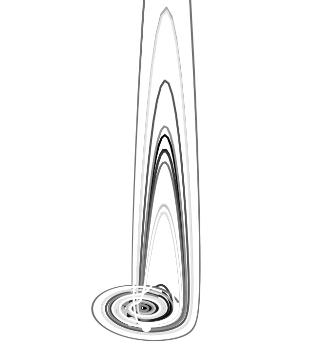
\includegraphics[width=8cm]{rossler}
  	\caption{Atractor de Rossler}
  	\label{rossler1}
  \end{figure}
  
 \section{Juego de la vida}
 \subsubsection{\large Simular el juego de la vida y estudiar su comportamiento emergente} 
  
  El juego de la vida es un autómata celular diseñado por el matemático británico John Horton Conway en 1970.
  
  Hizo su primera aparición pública en el número de octubre de 1970 de la revista Scientific American, en la columna de juegos matemáticos de Martin Gardner. Desde un punto de vista teórico, es interesante porque es equivalente a una máquina universal de Turing, es decir, todo lo que se puede computar algorítmicamente se puede computar en el juego de la vida.
    \begin{figure}
    	\centering
    	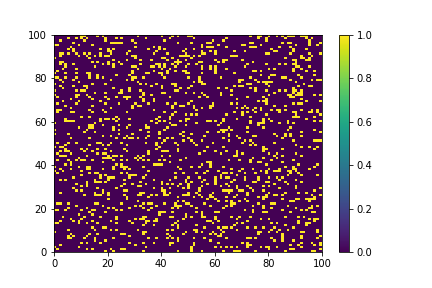
\includegraphics[width=8cm]{generation0}
    	\caption{Disposicion inicial: partimos de una distribucion aleatoria de puntos en una malla}
    	\label{gol1}
    \end{figure}
  \begin{figure}
  	\centering
  	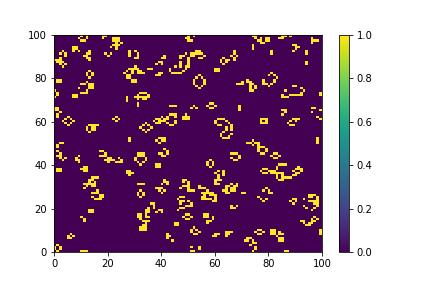
\includegraphics[width=8cm]{generation5}
  	\caption{Evolucion del juego de la vida tras 5 pasos temporale}
  	\label{gol2}
  \end{figure}
  \begin{figure}
  	\centering
  	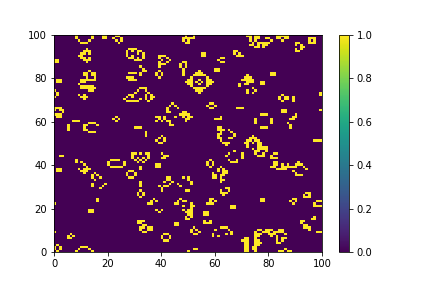
\includegraphics[width=8cm]{generation10}
  	\caption{Evolucion del juego de la vida tras 10 pasos temporales }
  	\label{gol3}
  \end{figure}
  Para profundizar un poco más en el trabajo se ha desarrollado un programa para detectar si patrones implementados generan naves espaciales.
  Las naves espaciales son patrones que reaparecen en otra posición tras completar su período. Esto es, son patrones que tras un número finito de generaciones vuelven a su estado original pero en una ubicación diferente.
  En este caso se han utilizado las reglas estándar. Tras 4 pasos temporales se localizó que la figura era una nave espacial (figuras \ref{gol4} y \ref{gol5})
   \begin{figure}
   	\centering
   	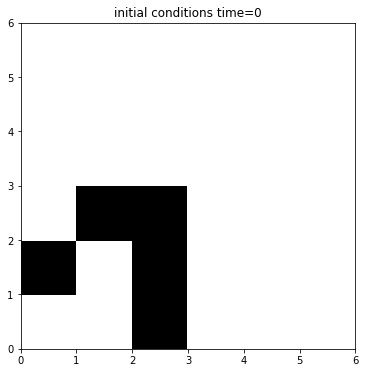
\includegraphics[width=8cm]{searcher_1}
   	\caption{Disposicion inicial encontrada como buena }
   	\label{gol4}
   \end{figure}
    \begin{figure}
    	\centering
    	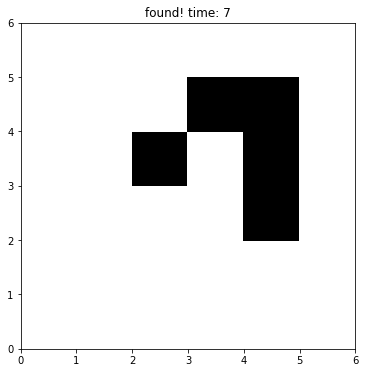
\includegraphics[width=8cm]{searcher_2}
    	\caption{Identidad identica transportadad tras 4 pasos temporales }
    	\label{gol5}
    \end{figure}
    Esta es la nave espacial más famosa, conocida como glider.
\subsubsection{\large Modelo pilas de arena}     
El modelo de pilas de arena es un modelo matemático diseñado para analizar y explicar el comportamiento de autoorganización crítica a través de la teoría de grafos y la teoría de autómatas celulares utilizando herramientas algebraicas.

Si consideramos un plano con una gran cantidad de arena al que se le va añadiendo un poco cada paso temporal, si la pendiente es muy alta, la arena tenderá a caer provocando una avalancha, pues es un estado insetable. Esto se poducirá hasta que todo llegue a un estado estable en cuanto a la pendiente.

Se pueden ver el resultado de las simulaciones en \ref{sand1},\ref{sand2},\ref{sand3}

 \begin{figure}
 	\centering
 	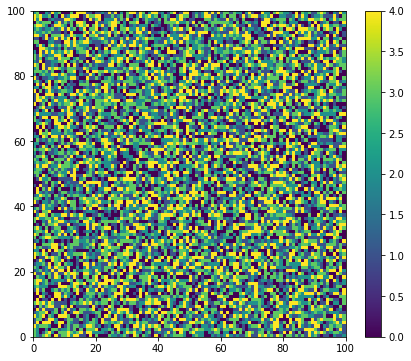
\includegraphics[width=8cm]{pila_arena_random}
 	\caption{Pila de arena con condiciones iniciales aleatorias  }
 	\label{sand1}
 \end{figure}
  \begin{figure}
  	\centering
  	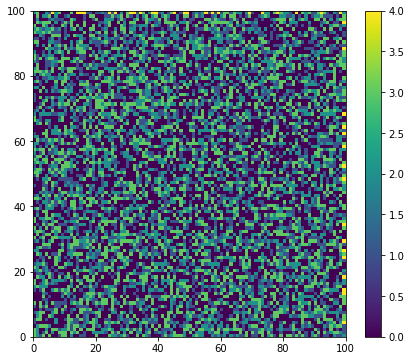
\includegraphics[width=8cm]{pila_arena_random_2}
  	\caption{Sin adicion y partiendo de \ref{sand1} vemos como el sistema tiene a producir avalanchas hasta nivelarse }
  	\label{sand2}
  \end{figure}

 \begin{figure}
 	\centering
 	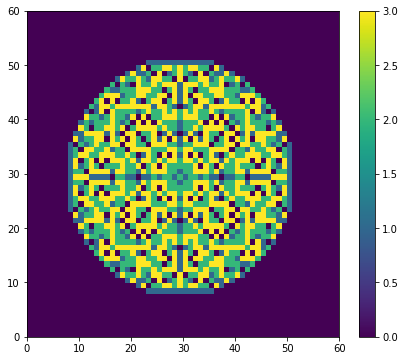
\includegraphics[width=8cm]{pila_arena}
 	\caption{Creacion de fractales cuando añadimos un goteo de arena en el centro durante 100 pasos de tiempo }
 	\label{sand3}
 \end{figure}


    
\subsubsection{\large Modelo hormiga de langton}    
Aunque no partía como ejercicio, buscando información sobre algunas de turing y el juego de la vida también he encontrado otra sencilla maquina con comportamientos emergentes que dejo a continuación.
La hormiga de Langton es un una máquina de Turing bidimensional con un conjunto de reglas muy sencillo, que sin embargo da lugar a comportamientos emergentes complejos.
 La hormiga de Langton clásica opera sobre una rejilla espacial cuadrada, en que cada celda puede estar en uno de dos estados (blanca o negra, 1 o 0, viva o muerta, etc). Fue inventada por Chris Langton en 1986 y su universalidad se demostró en el año 2000.
 
 La hormiga siempre está mirando en una de las cuatro direcciones cardinales y se mueve un cuadrado cada vez, de acuerdo con las siguientes reglas:
 \begin{itemize}
 	\item Si está sobre un cuadrado blanco, cambia el color del cuadrado, gira noventa grados a la izquierda y avanza un cuadrado.
 	\item Si está sobre un cuadrado negro, cambia el color del cuadrado, gira noventa grados a la derecha y avanza un cuadrado.
 \end{itemize}
 
   \begin{figure}
   	\centering
   	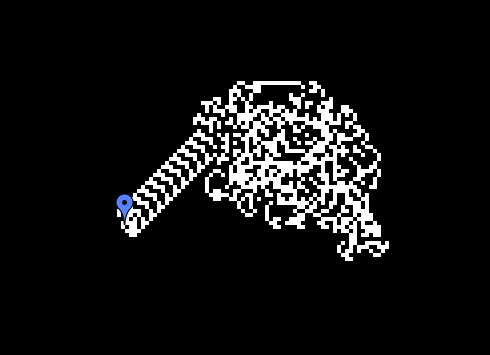
\includegraphics[width=8cm]{ant}
   	\caption{Hormiga tras 11000 pasos temporales. Las condiciones iniciales son nulas salvo la casilla de la hormiga }
   	\label{ant}
   \end{figure}
  



\section{Dimensiones de Haussdorf: variedades continuas y fractales}
\subsubsection{\large Demostrar que con la definición de dimension de Haussdorf se tiene (para variedades continuas:curva, superficie, y volumen) las dimensiones esperadas.} 

Partimos de la formula descrita en los apuntes, la dimension de Haussdorf ($D$) de una variedad viene determinada por:
\begin{equation}
D=\lim_{a\rightarrow 0}(\frac{-ln(N(a))}{ln(a)})
\end{equation}
donde $N(a)$ es el número mínimo de $esferas$ $d–dimensionales$ necesarias para cubrir por completo la variedad en cuestión.
Teniendo en cuenta que $d T \leq D \leq d$, donde $d$ es la dinemsion euclídea y $d_T$ e sla dimension topológica, sabemos de antemano que como todas nuestras variedades son continuas, el valor será $1,2,3$ para la curva, la superficie y le columen, respectivamente. Analizamos caso por caso: 
\begin{itemize}
	\item Curva continua:
	
	En este caso las $esferas$ $d–dimensionales$ son segmentos de longitud $2a$, por tanto, sea una curva continua con longitud $1$:
	\begin{equation}
	\begin{split}
	D=\lim_{a\rightarrow 0}(\frac{-ln(N(a))}{ln(a)})
	&=-\lim_{a\rightarrow 0}(\frac{ln(1/2a)}{ln(a)})\\
	=-\lim_{a\rightarrow 0}(\frac{\frac{d}{da}ln(1/2a)}{\frac{d}{da}ln(a)})
	&=-\lim_{a\rightarrow 0}(\frac{-1/x}{1/x})=1
	\end{split}
	\end{equation}
	\item Superficie continua:
	
	En este caso las $esferas$ $d–dimensionales$ son discos de radio $a$, por tanto, dada una superficie, podemos recubir su borde colocando esferas que abarcan una longitud de $2a$ a lo alto y a lo largo:
	
	\begin{equation}
	\begin{split}
	D=\lim_{a\rightarrow 0}(\frac{-ln(N(a))}{ln(a)})
	&=-\lim_{a\rightarrow 0}(\frac{ln(1/(2a)^2)}{ln(a)})\\
	=-\lim_{a\rightarrow 0}(\frac{\frac{d}{da}ln(1/4x^2)}{\frac{d}{da}ln(a)})
	&=-\lim_{a\rightarrow 0}(\frac{-2/x}{1/x})=2
	\end{split}
	\end{equation}
	
	\item Volumen continuo:
	
	En este caso las $esferas$ $d–dimensionales$ son esferas de radio $2a$, por tanto, dado un volumen continuo podemos recubir su borde colocando esferas que abarcan una longitud de $2a$ a lo alto, a lo ancho y a lo largo :
	\begin{equation}
	\begin{split}
	D=\lim_{a\rightarrow 0}(\frac{-ln(N(a))}{ln(a)})
	&=-\lim_{a\rightarrow 0}(\frac{ln(1/(2a)^3)}{ln(a)})\\
	=-\lim_{a\rightarrow 0}(\frac{\frac{d}{da}ln(1/8x^3)}{\frac{d}{da}ln(a)})
	&=-\lim_{a\rightarrow 0}(\frac{-3/x}{1/x})=3
	\end{split}
	\end{equation}
\end{itemize}


\subsubsection{\large Calcular la dimensión Hausdorff de los siguientes fractales: Conjunto de Cantor, la Isla de Koch, la Alfombra de Sierpinsky y la triangulo de Sierpinsky} 
 Atendiendo a la definición de las notas, tenemos que $$M\sim R^D$$
 donde D es la dimensión fractal. 
 Por tanto si desarrollamos obtenemos: 
$$D=\frac{log(M)}{log(R)}$$
Pasemos a analizar cada uno de los casos. 
\begin{itemize}
	\item Conjunto de cantor:
	
	en este caso tenemos una variedad de masa 1, de manera que en cada paso obtenemos dos subvariedades, estas subvariedades coinciden con la original si aumentamos la escala 3 unidades de la que tenemos, por tanto:  $$D=\frac{log(2)}{log(3)}$$
	
	\item Isla de Koch:
	
	en este caso tenemos una variedad cuya dimension D debe ser $1<D<2$. En esta figura si aplicamos un factor de multiplicacion 3 obtenemos 4 veces la seccion inicial que habíamos aumentado, por tanto:  $$D=\frac{log(4)}{log(3)}$$

	\item Alfombra de Sierpinsky:
	
	en este caso tenemos una variedad cuya dimension D debe ser $1<D<2$. Si aumentamos la figura por un factor 3, obtenemos 8 subvariedades identicas a la original , por tanto:  $$D=\frac{log(8)}{log(3)}$$
	
	\item triangulo de Sierpinsky:
	
	en este caso tenemos una variedad cuya dimension D debe ser $1<D<2$. Si aumentamos la figura por un factor 2, obtenemos 3 subvariedades identicas a la original , por tanto:  $$D=\frac{log(3)}{log(2)}$$
\end{itemize}





